%&pdflatex
\documentclass[12pt]{article}
\usepackage[margin=1.0in]{geometry}

\usepackage{g-util, g-uba, g-algo}
\usepackage{subfiles}

\begin{document}

\titulo{TP1: Técnicas Algorítmicas}
%\subtitulo{Técnicas Algorítmicas}
\fecha{21 de Septiembre de 2022}
\materia{Algoritmos y Estructuras de Datos III}
\integrante{Cappella Lewi, Federico Galileo}{653/20}{glewi@dc.uba.ar}
\integrante{Mallol, Martín Federico Alejandro}{208/20}{martinmallolcc@gmail.com}
\integrante{Teplizky, Gonzalo Hernán}{201/20}{gonza.tepl@gmail.com}
\integrante{Stemberg, Uriel Nicolás}{213/20}{uri.stemberg@gmail.com}
\maketitle

\newpage
\begin{abstract}
  Para este trabajo el enfoque será puesto en experimentar con distintas técnicas algoritmicas recursivas, con el fin de encontrar algoritmos más rápidos y eficientes que aquellos que emplean fuerza bruta. Mas allá de que en la mayoría de los casos sea imposible evitar una complejidad exponencial, se intentará acotar lo más posible el tiempo de cómputo de cada programa implementado en este trabajo. Se deben resolver tres ejercicios donde, cada uno de ellos se tratará sobre el comportamiento de una de estas tres técnicas en específico: backtracking, algoritmo goloso/greedy/miope (cualquiera de estas tres definiciones es válida), y por último, programación dinámica. \\
  \textbf{Palabras clave}: \textit{Fuerza Bruta}, \textit{Backtracking}, \textit{Greedy}, \textit{Programación Dinámica}, \textit{Complejidad Temporal}, \textit{Complejidad Espacial}.
\end{abstract}

\tableofcontents

%\newpage
%%&pdflatex
\documentclass[./main.tex]{subfiles}

\begin{document}

\section{Ejercicio 1: Robots On Ice}
\label{sec:ej1}

\subsection{Presentación}
\label{sec:ej1-intro}

\paragraph{} La primer consigna plantea resolver el problema \textit{UVa 1098, Robots On Ice}\footnote{\url{https://onlinejudge.org/index.php?option=onlinejudge&Itemid=8&page=show_problem&problem=3539}}. En el que se busca contar todos los caminos posibles dentro de un mapa que cumplan ciertas condiciones.

\paragraph{} El mapa es una grilla rectangular de tamaño \(n \times m\), con \(2 \leq n, m \leq 8 \in \mathbb{N}\). Y los caminos empiezan en la posición \((0, 0)\) y terminan en la posición \((0, 1)\), teniendo que pasar en orden por tres posiciones, o check-ins, en momentos equidistantes de el camino. \\
Tanto \(n, m\), y los check-ins, son parámetros de entrada que el programa lee del standard input. Y resultado se devuelve por el standard output. \\
\indent Dentro del mapa sólo es posible moverse en las cuatro direcciones cardinales, sin poder repetir posiciones previamente pisadas.

\subsection{Algoritmo}
\label{sec:ej1-algo}

\paragraph{} Para resolver este problema utilizamos \textbf{backtracking}, armando a fuerza bruta todos los caminos posibles, descartando los que no cumplan con las condiciones pedidas, y contando los que sí. \\
\indent El algoritmo empieza en la posición inicial dada, y prueba moverse en cada dirección. Si el movimiento fue legal, cumple con las restricciones, y no rompe las restricciones a futuro (ver \textbf{\ref{sec:ej1-podas} Podas}), entonces continúa recursivamente, ahora probando moverse desde esta nueva posición. \\
\indent Como para cada posición se prueban cuatro movimientos, la complejidad temporal es \(\bigO{4^{n*m}}\).

\subsubsection{Podas}
\label{sec:ej1-podas}

\paragraph{} Como parte del algoritmo, implementamos dos tipos de podas para descartar caminos:
\subparagraph{Legales (o de Factibilidad)}
\begin{itemize}
  \item El movimiento no se sale del mapa. Osea, se mueve a una posición \((i, j)\) con alguna de las dos coordenadas fuera de rango).
  \item No se pasó ya por el casillero de destino. Para esto llevamos registro de los casilleros por los que se pasó en una matriz de \(n \times m\) booleanos.
\end{itemize}

\subparagraph{Restrictivas y Preventivas (o de Optimalidad)}
\begin{itemize}
  \item El casillero de destino. Como los check-ins tienen que ser visitados en tiempos equidistantes necesitamos que en el paso \(\dfrac{n*m*i}{4}\) estemos en el \(i\)-ésimo check-in (para \(0 \leq i \leq 4 \in \mathbb{N}_0\), contando a las posiciones \((0, 0)\), y \((0, 1)\) como check-in 0 y 4 respectivamente).
  \item Como sólo nos podemos mover de a un casillero por paso y sólo en las 4 direcciones, nos queda que entre las posiciones \((i, j)\) y \((l, k)\) se tienen mínimo \(|l-i| + |k-j|\) pasos, que es \textit{distancia Manhattan}. Por lo que nos fijamos que estemos a menos de \(|l-i| + |k-j|\) pasos del paso necesario para el check-in \((k, j)\) (con \((i, j)\) la posición actual).
  \item Como no podemos pasar dos veces por el mismo casillero, nos fijamos de no cortar en dos partes desconectadas al mapa. Esto sucedería cuando nos podemos mover tanto a izquierda como a derecha, pero no hacia arriba o hacia abajo, y simétrico pudiendo moverse hacia arriba y hacia abajo, pero no a derecha o izquierda (ver Fig. \ref{fig:ej1-mitad}).
\end{itemize}

\begin{figure}[H]
\centering

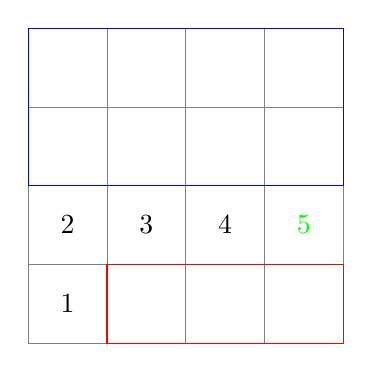
\begin{tikzpicture}
  \draw[step=1cm,gray,very thin] (0,0) grid (4,4);
  \draw (0.5, 0.5) node{1};
  \draw (0.5, 1.5) node{2};
  \draw (1.5, 1.5) node{3};
  \draw (2.5, 1.5) node{4};
  \draw[green] (3.5, 1.5) node{5};
  \draw[red] (1, 0) rectangle (4, 1);
  \draw[blue] (0, 2) rectangle (4, 4);
\end{tikzpicture}

\caption{En esta figura se ve un camino posible en un mapa de \(4 \times 4\), y las dos areas desconectadas del mapa marcadas en rojo y en azul.}
\label{fig:ej1-mitad}
\end{figure}

\end{document}


%\newpage
%\documentclass[./main.tex]{subfiles}

\begin{document}

\section{Ejercicio 2: Watering Grass}
\label{sec:ej2}

\subsection{Presentación}
\label{sec:ej2-intro}

\paragraph{} El segundo ejercicio presenta el problema \textit{UVa 10382, Watering Grass}\footnote{\url{TODO: URL}}. Que es un problema de combinatoria y minimización, buscando usar la mínima cantidad de aspersores para cubrir completamente un cuarto.

\paragraph{} El cuarto está definido como un rectángulo de largo \(l\) y ancho \(w\), con \(l, w \in \mathbb{N}_0\), y \(n\) aspersores, cada uno cubriendo un círculo de radio \(r_i\) desde la posición \((x_i, \frac{w}{2})\), con \(0 \leq x_i \leq l \in \mathbb{N}_0\). \\
\(l, w, n\), y cada \(r_i, x_i\) son datos que entran por el standard input. Y el resultado se devuelve por el standard output.

\subsection{Algoritmo}
\label{sec:ej2-algo}

\paragraph{} El problema requiere calcular el area del rectángulo que cada aspersor cubre. Pero se puede ver que de cada aspersor sólo nos importa el area rectangular entre los puntos donde interseca con el rectángulo del cuarto, ya que el area cubierta afuera sólo puede ser ocupada por el area rectangular de otro aspersor o dejaría un area sin cubrir por ningún aspersor (ver Figura \ref{fig:two-sprinlers}). \\
\indent Entonces los aspersores con radio \(r_i < \frac{w}{2}\) pueden ser ignorados, ya que no llegan a intersecar con el lado del rectángulo. Y para los aspersores que quedan se los considera no como círculos, sino como su rectángulo subyacente (ver Figura \ref{fig:simple-sprinkle}).

%TODO: Figura rectángulo y círculos

\paragraph{} Partiendo de esa simplificación armamos un algoritmo goloso que primero ordena los aspersores según menor \(izq_i\). Y luego busca el \(i_0\) de izquierda a derecha que tenga \(izq_{i_0} \leq 0\) y que maximice la distancia entre 0 y \(der_{i_0}\), para después repetir este paso, pero buscando \(i_1\) tal que \(izq_{i_1} \leq der_{i_0}\), y maximice la distancia entre \(der_{i_0}\) y \(der_{i_1}\), y así hasta, o no haber más aspersores (caso que no se puede resolver), o haber llenado el cuarto (caso que se encontró la solución optima, ver \textbf{\ref{sec:ej2-dem} Demostración}). \\ %TODO: Explicar qué es izq_i, y der_i
En esencia, repitiendo el problema habiendo avanzado hacia cubrir todo el cuarto.

\paragraph{} Como miramos cada aspersor una vez, el algoritmo resuelve el problema en \(\bigO{n}\) pasos, aunque tiene el overhead \(\bigO{n\ log(n)}\) de ordenar los aspersores. Por lo que el problema lo resolvemos en \(\bigO{n\ log(n)}\) pasos. %TODO: Complejidad de cálculos

\subsection{Demostración}
\label{sec:ej2-dem}

\paragraph{} Para la demostración planteamos:
\begin{itemize}
  \item \(izq_i\), y \(der_i\) como los lados izquierdo y derecho del rectángulo subyacente del aspersor \(i\). %TODO: Se va a más arriba
  \item A \(\mathcal{S}\) el espacio de soluciones. Con \(S = s_1, \ldots, s_m \in \mathcal{S} \mid izq_{s_1} \leq 0 \land der_{s_m} \geq l \land der_{s_i} \leq izq_{s_{i+1}}\). \\
  Se puede ver que para una instancia del problema, todas las soluciones \(S \in \mathcal{S}\) tienen el mismo largo, ya que para ser solución tienen que minimizar su largo. 
  \item A \(G_k = g_1, \ldots, g_k\) la secuencia golosa luego de haber hecho \(k\) decisiones golosas. O sea que, \(izq_{g_1} \leq 0 \land g_{i+1} = max_j\{der_j - der_{g_i} \mid der_{g_i} \leq izq_j\}\).
\end{itemize}

Con esto, planteamos la estructura de cada \textbf{subproblema} y \textbf{decisión golosa} \textit{i} a resolver: \newline

-\textit{Subproblema i}: Hallar la mínima cantidad de aspersores requeridos con el que podamos cubrir el  rectángulo de forma tal que lo hagamos desde el extremo \textit{i} (visto horizontalmente) hasta el final del rectángulo.\newline

-\textit{Decisión golosa i}: De todos los aspersores cuyo límite izquierdo sea menor o igual a \textit{i}, es decir, que empiecen en \textit{i}, que es hasta donde tenemos cubierto, o antes, tomamos el aspersor que sea de máximo cubrimiento, lo cual según definimos será aquel que maximice \textbf{limiteDer(aspersor) - limiteIzq(aspersor)}. \newline

\paragraph{} Entonces queremos probar: \begin{itemize}
  \item[\textbf{1)}] Cualquier solución óptima \(S = s_1, \ldots, s_m\) puede ser modificada para obtener una solución óptima que use una decisión golosa.
  \item[\textbf{2)}] La secuencia \(G_k\) puede ser extendida a una solución óptima.
\end{itemize}

\paragraph{} Primero probamos \textbf{1)}, que se puede ver porque si tomamos la solución ópitma \(S = s_1, \ldots, s_{k-1}, s_k, s_{k+1}, \ldots, s_m\) y armamos \(S' = s_1, \ldots, s_{k-1}, g_k, s_{k+1}, \ldots, s_m\) tal que \(g_k = max_j\{der_j - der_{s_{k-1}} | der_{s_{k-1}} \leq izq_j\}\), \(S'\) sigue siendo una solución óptima ya que \(der_{s_{k-1}} \leq izq_{g_k}\) y \(der_{g_k} \geq der_{s_k}\) por lo que \(der_{g_k} \leq izq_{s_{k+1}}\). \\
De esta forma se puede seguir modificando a \(S\), hasta haber tomado \(m\) decisiones golosas y se llegaría a una secuencia golosa.

\paragraph{} Y ahora probamos \textbf{2)} usando el método inductivo. \begin{itemize}
  \item Definimos la proposición \(P(k) \equiv G_k\) se puede extender a una solución óptima.
  \item[\textbf{Caso base:}] \(P(0)\). Es trivial porque \(G_0 \equiv \emptyset\).
  \item[\textbf{Paso inductivo:}] \(P(k) \Rightarrow P(k+1)\). Si \(k+1 > m\) entonces es trivial, ya que \(G_k\) ya sería la solución óptima. \\
    Lo revisamos entonces para \(k+1 \leq m\). Por \textbf{HI} tenemos que \(G_k = g_1, \ldots, g_k\) es extensible a una solución \(S = g_1, \ldots, g_k, s_{k+1}, \ldots, s_m\). Como \(S\) es solución sabemos que \(der_{g_k} \leq izq_{s_{k+1}} \land izq_{s_{k+2}} \leq der_{s_{k+1}}\), por lo que si tomamos \(g_{k+1} = max_j\{der_j - der_{g_k} \mid der_{g_k} \leq izq_j\}\) se mantiene que \(der_{g_k} \leq izq_{g_{k+1}}\), y como \(der_{s_{k+1}} \leq der_{g_{k+1}}\) se mantiene que \(izq_{s_{k+2}} \leq der_{g_{k+1}}\). Por lo que \(G_{k+1}\) es extensible a una solución. \done %TODO: Mencionar qué pasa con P(m)
\end{itemize}

\end{document}


%\newpage
%\documentclass[./main.tex]{subfiles}

\begin{document}

Por último, en el tercer ejercicio se debe trabajar con una variante del anterior. 
\newline

Vamos a contar con un terreno de $l \cdot w$, siendo nuevamente $l$ el $largo$ y $w$ el $ancho$, pero ahora el planteo del problema es un poco distinto. Se vuelve a tener a disposición una cantidad $n$ de aspersores con su $radio "r"$ y su posición \(pos\), pero se les agrega un atributo más, su $costo "c"$. Aquí radica la escencia del problema, ya que en vez de tener que encontrar la menor cantidad posible de aspersores que puedan regar todo el terreno, se debe encontrar el conjunto de aspersores que pueda \textbf{cubrir todo el terreno} y que \textbf{su costo total sea el mínimo posible} (entre todos los conjuntos de aspersores que pueden cubrir el jardín). Como el algoritmo que emplearemos arroja el mínimo costo posible y no el conjunto de aspersores, si hay más de un conjunto de aspersores que cumplan con el mínimo costo no altera el resultado final de la función.
\newline

Para resolver este problema en particular, se tomó como técnica algorítmica la \textbf{"Programación Dinámica"}, porque se buscó evitar que la función que soluciona este ejercicio no resuelva el mismo problema varias veces. Si esto ocurriera, se perdería mucho tiempo ejecutando cosas a las cuales ya se le conocen su valor.
\newline

A la hora de plantear el problema, tomamos un camino distinto al de la resolución \(golosa\) anteriormente mencionada. En vez de tener una \textbf{cola de prioridad} donde los aspersores están ordenados de mayor a menor según su prioridad (a menor límite izquierdo, mayor la prioridad), empleamos un \textbf{vector} para posicionarlos. Primero cargamos a los aspersores en este en base a su posición de llegada (es decir, el primero en ser cargado vía consola irá a la primer posicion, el segundo a la segunda, y así hasta el aspersor número "n"). Una vez que el vector estuvo listo, se lo ordenó con $mergesort$ (coste \textbf{O(n $\cdot$ log n)}) nuevamente según su límite izquierdo en el jardín. La única diferencia es que ahora, para poder acceder a un aspersor, podemos hacerlo con su índice en \textbf{O(1)} sin alterar las propiedades del vector, mientras que con la cola de prioridad, sí o sí deberíamos desencolar sus elementos para llegar a determinada posición i, con i \(\in \lbrace 1, \ldots, |cola| \rbrace\).
\newline

Con nuestro conjunto ordenado de aspersores ya conocido, llamémoslo $\mathbb{A}$, donde $a_i$ es el \(i\)-ésimo aspersor, especificamos el problema. Se busca encontrar la solución X tal que $X \subset \mathbb{A}$ y X riega todo el jardín y $\forall Y \subset \mathbb{A}$ que riegue todo el jardín, $costeTotal(Y) = \sum_{i=1}^{|Y|}costo(y_{i}) \geq \sum_{i=1}^{|X|}costo(x_{i}) = costeTotal(X)$. Veamos cómo es la función que resuelve esta problemática.
\newline

Se llama $\textbf{f(i,j) = costeTotal(X)}$. Tener en cuenta que, para todas las funciones a continuación con los parametros $i,j$, estos corresponden al \(i\)-ésimo y \(j\)-ésimo aspersor respectivamente. Y además, el $aspersor_i$ siempre está \textbf{a la derecha} del $aspersor_j$. Con esto en mente, la función principal (junto con sus auxiliares) es la siguiente: 
\newline
    %minimoCoste: Nat x Int --> Nat
\begin{equation}
 \label{función para el mínimo coste de aspersores}
 f(i,j) = \left\{
       \begin{array}{ll}
     0      & \mathrm{si\ } estaLleno(j) \\
     -1  & \mathrm{si\ } noSeLlenara(i,j) \\
     f(i+1,j)     & \mathrm{si\ } noSeLlenara(i+1,i) \\
     f(i+1,i) + costo(i)     & \mathrm{si\ } noSeLlenara(i+1,j) \\
     min((f(i+1,j), f(i+1,i) + costo(i))) & cc
       \end{array}
     \right.
\end{equation}

   % ANIMATE A PROCEDER QUE PEDAZO DE COMUNISTA LOKO JAJAJAJAJA ESTOY DANDO MI VIDA POR ESTE TP NO DUDO QUE TU DEMOSTRACION SERA FABULOSA VOY A ESO, QUE ME ESPERAN LOS SOCKETS DSPS GOOOOOD LA CLASE DE HOY PINTA PARA MASACRE, QUE LA DISFRUTEN LOS QUE VAN. DIOS NOS LIBRE

%noSeVaALlenar(i,j) = | True si (i = n and !estaLleno(j)) or noPuedoLlenarloAhora(i,j))
                         %| False si estaLleno(j)
                         %| noSeVaALlenar(i+1,j) or noSeVaALlenar(i+1,i)
\begin{equation}
 \label{función para ver si se va a llenar el terreno}
 noSeLlenara(i,j) = \left\{
       \begin{array}{ll}
     True      \phantom{aaaaaaa} \mathrm{si\ } (i = n \land \neg estaLleno(j)) \lor noPuedoLlenarlo(i,j)) \\
     False   \phantom{aaaaaal} \mathrm{si\ } estaLleno(j) \\
     noSeLlenara(i+1,j) \lor noSeLlenara(i+1,i) \phantom{aaaa}  \mathrm{cc\ }  \\
       \end{array}
     \right.
\end{equation}

\begin{equation}
 \label{función para ver si se puede llenar el terreno entre medio de los aspersores i,j}
 noPuedoLlenarlo(i,j) = limiteDerecho(aspersores_j) < limiteIzquierdo(aspersores_i). 
\end{equation}

\begin{equation}
 \label{función para ver si con el aspersor actual se cubre el final del terreno}
 estaLleno(j) = (l = 0) \lor ((j \neq -1) \land \neg(limiteDerecho(aspersores_j) < l) 
\end{equation}


La función se resuelve con \textbf{f(0,-1)} y devuelve el mínimo coste de un conjunto de aspersores que pertenece a todos aquellos conjuntos de aspersores que riegan completamente el terreno. Es decir, si $\mathbb{O}$ = $\lbrace o_1,...,o_m  \rbrace$ la solución óptima, siendo $\mathbb{S}$ el conjunto de soluciones posibles, entonces se tiene $\mathbb{O} \in \mathbb{S}$ / $f(0,-1)$ = $\sum_{i=1}^{|\mathbb{O}|}costo(o_{i})$.
\newline

Esta funcion tiene este comportamiento ya que existen dos casos, uno en el que el aspersor actual $a_i$ forma parte de un conjunto óptimo $\mathbb{O}'$ de $r$ elementos, y otro donde no lo hace. Si forma parte, la solución al problema será $(\sum_{i=1}^{r-1}costo(o_{k}')) + costo(a_i)$. Mientras que si no lo hace, entonces el costo de la solucion optima $\mathbb{O}'$  de $r$ elementos es $\sum_{i=1}^{r}costo(o_{k}')$. Siempre y cuando exista ese óptimo, lo elegiremos, mientras que si no hay solución al problema, es decir, el conjunto solución $\mathbb{S}$ está vacío, se devolverá $-1$.  
\newline

Ahora bien, \textbf{¿vale la pena memoizar?} Si la función es correcta se puede simplemente programar y listo. El problema ya se resuelve. Sin embargo, el inconveniente que se presenta es que existe la superposición de subproblemas en este algoritmo, ya que calculamos muchas veces instancias ya resueltas. Por esto mismo, empleamos \textbf{Programación Dinámica}. Esto se debe a que la cantidad de llamados recursivos es $\Omega(2^{n}????????)$, mientras que la cantidad de subinstancias es ${O(n^2)}$. Por lo que presentamos una cantidad de llamadas exponencial mientras que las subinstancias son mucho menores al ser polinomial. Recordando que $n$ es la cantidad de aspersores \textit{válidos}\footnote{Llamamos a un aspersor \textbf{válido} si su diámetro de riego puede cubrir el ancho del terreno.} dentro del terreno.
\newline

Para la memoización primero optamos por el enfoque \textbf{Top-Down}. Empleamos como estructura para guardar los datos ya calculados una matriz de $n+1 \times n+1$. Este algoritmo tiene una $complejidad$ $temporal$ y $espacial$ de $O(n^{2})$ (por la dimensión de la matriz). Su pseudocódigo es el siguiente:
\newline

% ME FALTA DE ACA PARA ABAJO!
\begin{algorithm}
\caption{menorCostoTopDown(A):}
\begin{algorithmic} 
\STATE Se inicializa M de $n+1 \times n+1$ con \(\bot\)
\RETURN f(0,-1) tal que
\STATE \textbf{f(i,j):}
\IF{estaLleno(j)}
\RETURN 0
\ENDIF
\IF{noSeLlenara(i,j)}
\RETURN -1
\ENDIF
\IF{M[i,j] = \(\bot\)}
\IF{noSeLlenara(i+1,i)}
\STATE M[i,j] \(\leftarrow\) f(i+1,j) 
\ENDIF
\ENDIF
\STATE $i \leftarrow 0$
\STATE $cubierto \leftarrow 0$
\STATE $minAspersores \leftarrow 0$
\RETURN $minAspersores$
\end{algorithmic}
\end{algorithm}

Luego fuimos por un enfoque \textbf{Bottom-Up} para poder comparar ambos métodos y ver realmente cuál es el que ahorra más tiempo de ejecución al eliminar pasos redundantes en el árbol recursivo. Se volvió a disponer, en principio, de una matriz de $n+1 \times n+1$, pero en vez de tener un algoritmo \textbf{recursivo}, este es \textbf{iterativo}. Se itera a la matriz de \textit{izquierda a derecha} y de \textit{abajo a arriba}. Es decir, cuando estamos parados en una \textit{fila i}, la recorremos desde su $primera$ posición hasta su \(i\)-ésima posición. Esto se repite partiendo desde la \textit{n+1-ésima fila} hasta la $primera$. Como en la funcion $f$ anteriormente mencionada el parámetro $i$ nunca es mas grande que el parámetro $j$, no se visitan aquellas celdas donde el número de la fila sea mayor al de la columna. Para finalizar con la explicación, el algoritmo queda con \textit{complejidad temporal y espacial O(n$^{2}$)} (por la matriz también). Teniendo esto en mente, mostramos el algoritmo:
\newline

PSEUDOCODIGO
\newline

Al finalizar la implentación \textbf{Bottom-Up} notamos algo clave. Se puede \textit{ahorrar espacio} con la estructura de memoización. No hace falta tener una matriz de $n+1 \times n+1$ para representar todas las soluciones, (tanto parciales como candidatas). Al no tener que reconstruir la solución ya que sólo se debe devolver el coste y no los aspersores que pertenecen al conjunto óptimo, podemos \textbf{desechar la matriz} y tener como estructura de memoización un \textbf{vector} de longitud $n+1$, guardando solamente la \textit{fila anteriormente calculada} y no todas las filas anteriores como sucedía con la matriz. Esto no mejora la \textit{complejidad temporal} pero sí la $espacial$, dejándola en $O(n)$ en vez de O(n$^{2}$). Una mejora considerable en utilización de memoria. Su implementación quedó de la siguiente forma:
\newline

PSEUDOCODIGO
\newline

COMPARACION DE TIEMPOS DE EJECUCION ENTRE TOP-DOWN Y BOTTOM-UP PARA ELEGIR A UN GANADOR.
\newline

CONCLUSI\'ON

%% Hablar de por que la funcion funciona, luego del enfoque top down, despues el bottom up con matriz, y luego el bottom up sin matriz.

\end{document}


%\newpage
%\begin{thebibliography}{1}
%
%\bibitem{blabla} https://www.blablabla.com/blabla/
%\bibitem{blabla} https://www.blablabla.com/blabla/
%\bibitem{blabla} https://www.blablabla.com/blabla/
%
%\end{thebibliography}

\end{document}
